\documentclass[russian,utf8,pointsubsection,emptystyle
,reduceheight=5mm
]{eskdtext}
\usepackage{eskdchngsheet}
\usepackage{eskdplain}
\usepackage[T2A]{fontenc}
\usepackage{amstext}
\usepackage{amsmath}
\usepackage{listings}
\usepackage{wrapfig}
\usepackage{subfig}
\usepackage{longtable}

\ESKDdepartment{Московский Государственный Университет им.~М.В.~Ломоносова}
\ESKDcompany{Факультет Вычислительной Математики и Кибернетики

Кафедра Автоматизации Систем Вычислительных Комплексов}
\ESKDtitle{Разработка и реализация многопрофильной системы фильтрации спама на основе методов машинного обучения\\
\small{\textup{дипломная работа}}
}
\ESKDauthor{Петров Александр Владимирович}
\ESKDdate{2011/04/07}
\renewcommand{\ESKDtheTitleFieldII}{
\begin{center}
  
\includegraphics{msu}
\end{center}
}
\renewcommand{\labelitemi}{$\bullet$}
\renewcommand{\labelenumi}{\arabic{enumi}.}
\renewcommand{\ESKDtheTitleFieldIV}{
\parbox[r][4cm]{4cm}{}

\ESKDtheTitle}
\renewcommand{\ESKDtheTitleFieldVIII}{
\parbox[r][2.5cm]{5cm}{}

\begin{flushright}
  \parbox[r]{8cm}{
    \normalsize
	\textbf{Автор}

    \ESKDtheAuthor

    Группа 522

    кафедра АСВК, ЛВК

    \textbf{Научный руководитель}

    Герасёв Александр Витальевич
  }
\end{flushright}

}

\renewcommand{\ESKDtheTitleFieldX}{Москва \ESKDtheYear}

\usepackage[unicode]{hyperref}
\addtolength{\textwidth}{-0.5cm}

\begin{document}
\maketitle
\newpage
\section*{Аннотация}

%Аннотация (не более пол-страницы) содержит формулировку задачи и основных результатов

Данная работа посвящена задаче классификации прецедентов, образующих связные множества, возникающей при классификации результатов измерений в узлах некоторой сетки. Объектам в исходном непрерывном пространстве соответствуют связные области измерений (прецедентов) в дискретном пространстве узлов сетки. Частным случаем этой задачи является задача классификации данных лазерной локации.

Из-за отсутствия информации о форме и расположении объектов данная задача традиционно решается либо независимой классификацией прецедентов (с введением коллективных признаков), либо с использованием специфичных для свой области применения алгоритмов выделения объектов. В данной работе рассматривается подход, основанный на выделении границ объектов путем предварительной классификации и поиска связных областей прецедентов одного класса.

В результате работы была разработана экспериментальная система многоэтапной классификации данных лазерной локации. Серия экспериментов, проведенных с помощью этой системы, показала увеличение качества классификации.



\tableofcontents

\newpage
\section{Введение}

%Введение должно описывать предметную область, к которой относится задача, решаемая в дипломной работе,
% содержать неформальное ее описание;


\subsection{Задача фильтрации спама}
Данная работа посвящена фильтрации спама. Под спамом обычно понимают массовую рассылку сообщений, как то рекламные материалы приходящие по обычной почте, SMS,  системы обмена мгновенными сообщениями,  электронной почте.

Электронная почта в настоящее время является одним из основных способов общения. В протокол доставки электронной почты при его разработке не были включены никакие средства проверки подлинности личности отправителя, что существенно облегчило рассылку  сообщений. Кроме того, поскольку копирование электронного сообщения практически бесплатно, при использовании электронной почты проблема спама стоит особо остро. В данной работе под термином спам будет подразумеваться нежелательная электронная почта, то есть такая почта, которую пользователь не хотел бы получать даже зная о факте её отправки.

Термином легитимная почта мы будем обозначать электронные письма, не являющиеся спамом.

Так как получение нежелательной почты отвлекает пользователей электронной почты и создает ненужную нагрузку на сеть, со спамом необходимо бороться. С момента появления спама было придумано множество методов позволяющих отличить спам от легитимной почты. Перечислим некоторые классы этих методов:
\begin{itemize}
\item Методы, использующие информацию о сетевом соединении. В своей работе они анализируют IP-адреса, доменные имена и другую информацию на сетевом уровне.
\item Методы работающие на уровне протокола передачи электронной почты. Эти методы используют особенности протокола передачи почтовых сообщений (SMTP)  и точность его соблюдения клиентом.
\item Анализ заголовков и тела письма. Эти методы используют информацию содержащуюся в самом письме: комбинации заголовков, ключевые слова, соответствие регулярным выражениям. Могут применяться различные статистические методы.
\end{itemize}

\subsection{Статистические методы}

Эти методы представляют  из себя «черный ящик», получающий на вход письмо, и на выходе возвращающий оценку принадлежности этого письма к спаму. Внутри черного ящика выполняется алгоритм, выдающий оценку для письма в зависимости от некоторых статистических данных. Совокупность таких данных для некоторого адресата будем называть профилем.

Профиль строится  при помощи обучающей выборки – некоторого количества сообщений, для которых известно являются они спамом или легитимной почтой. Обучением статистического метода называется процесс построения профиля по обучающей выборке. Поскольку постоянно появляются новые виды спама и легитимной почты, необходимо уметь перестраивать профиль пользователя с учетом новых данных. Для некоторых алгоритмов необходимо полностью повторять процесс обучения, однако существуют алгоритмы, в которых можно использовать информацию полученную на ранних этапах добавив к ним новые знания. Процесс добавления в профиль новой информации называется дообучением.

Существует два подхода к построению профиля пользователя , необходимого для работы статистических методов:

\begin{itemize}
\item В обучающей выборке содержатся письма от всех пользователей. В этом случае при добавлении нового пользователя в систему он сразу может начинать пользоваться фильтром, не помечая приходящие к нему письма как спам или  легитимная почта. Однако возникает другая проблема, связанная с тем, что схожие письма для одних пользователей являются спамом, а для других легитимной почтой. (Например, менеджер вполне может получать письма с коммерческими предложениями, при этом если такие письма получает программист, то они почти наверняка являются спамом.)
\item Все письма из обучающей выборки принадлежат одному пользователю. В этом случае алгоритм работает достаточно хорошо (отсеивая практически весь спам, при этом вероятность ложного срабатывания достаточно мала). Однако, для того, чтобы алгоритм начал работать пользователь должен получить и добавить в свою обучающую выборку достаточно большое количество спама или легитимной почтой.
\end{itemize}

Все существующие на сегодняшний день открытые средства фильтрации спама используют либо первый, либо второй подход к фильтрации. Данная работа посвящена разработке третьего подхода, комбинирующего достоинства этих методов. В этом подходе должны строиться профили для каждого пользователя  и некоторые общие профили для групп пользователей. При классификации письма мы будем пользоваться некоторой комбинацией профилей. Такой подход мы будем называть многопрофильным.

\subsection{Размещение системы фильтрации  спама}
Фильтрацию спама можно проводить либо на стороне клиента, либо на стороне сервера.  При фильтрации на стороне клиента почтовый клиент скачивает письмо с сервера, после этого классифицирует почту.
При фильтрации на стороне сервера письмо классифицируется до передачи его в почтовый клиент пользователя. При этом пользователь может даже не скачивать письмо. Многопрофильную фильтрацию можно провести можно произвести только на стороне сервера, т. к. только на стороне сервера хранится информация,  необходимая для построения множества профилей пользователей.

\subsection{Методы машинного обучения}
Алгоритм, реализующий статистический метод по своей сути реализует тот или иной метод машинного обучения.
Машинное обучение – это научная дисциплина, изучающая построение алгоритмов, способных обучаться. При помощи машинного обучения решаются такие задачи как восстановление регрессии, кластеризация, классификация, прогнозирование.

Задача фильтрации спама является задачей классификации, нужно определить принадлежность письма к одному из классов: спам или легитимная почта.

Формально задача классификации ставится следующим образом: Имеется множество объектов (ситуаций), разделённых некоторым образом на классы. Задано конечное множество объектов, для которых известно, к каким классам они относятся. Это множество называется обучающей выборкой. Классовая принадлежность остальных объектов не известна. Требуется построить алгоритм, способный классифицировать произвольный объект из исходного множества. Классифицировать объект – значит указать номер(или наименование) класса, к которому принадлежит объект. Классификация объекта – номер или  наименование класса, выдаваемое алгоритмом классификации в результате его применения к данному конкретному объекту.

Обучением называется процесс постройки алгоритма классификации по обучающей выборке. Дообучение – процесс перестроения алгоритма классификации после добавления в обучающую выборку новых объектов. Для многих алгоритмов их не приходится перестраивать их с ноля, можно воспользоваться информацией полученной при ранних этапах обучения. Такие алгоритмы называются дообучаемыми.

Задачу классификации можно поставить вероятностно. В этом случае вместо класса объекта алгоной раритм должен выдавать не конкретный класс, а вероятность принадлежности объекта тому или иному классу.

Существует большое множество методов машинного обучения, обзор которых будет приведен в данной работе.

\newpage
\section{Цели работы и постановка задачи}

% Постановка задачи должна содержать формулировку задачи в рамках определенной модели
% предметной области, к которой относится решаемая задача, требования к искомому
% -решению в терминах используемой модели предметной области

Данная работа имеет две основные цели:
\begin{itemize}
\item Реализовать в рамках так из свободных антиспам-систем фильтрацию почты, основанную на методе опорных векторов.
\item Разработать и реализовать в рамках той же системы многопрофильную фильтрацию, основанную на методе опорных векторов.
\end{itemize}

Для этого предлагается решить следующие подзадачи:
\begin{enumerate}
\item  Провести обзор существующих открытых систем фильтрации спама и выбрать средство для расширения. 
\item В рамках выбранного средства реализовать фильтрацию спама, основанную на методе опорных векторов.
\item Разработать на базе метода опорных векторов метод, который позволит классифицировать почтовые сообщения по нескольким профилям.
\item Реализовать данный метод в рамках выбранного ранее средства.
\item Провести экспериментальное исследование на тестовых наборах
\begin{itemize}
    \item SpamAssassin public corpus
    \item CEAS 2008 Live Spam Challenge Laboratory Corpus
\end{itemize}
\end{enumerate}

Разрабатываемое средство должно удовлетворять следующим требованиям:
\begin{itemize}
\item должно распространяться под свободной лицензией;
\item должно работать демоном на сервере;
\item может быть интегрировано в большинство распространенных MTA;
\item в случае работы для одного пользователя качество классификации не хуже чем у наивного байесовского классификатора;
\item в случае работы для нескольких пользователей в режиме многопрофильной фильтрации качество классификации лучше чем у наивного байесовского классификатора;
\item производительность классификации должна быть сравнима с байесовскими методами.
\end{itemize}

\newpage
\section{Обзор предметной области}
\label{review}

\subsection{Методы машинного обучения} 
\label{ML}
\subsubsection{Обучение по прецедентам}
Пусть есть неизвестная функция $F: X -> Y$, переводящая объекты
множества $X$ в объекты множества $Y$, причем для некторых $x_1, x_2, ... x_n$ известны соответсвующие им значения $y_1 = F(x_1), y_2 = F(x_2), ... y_n = F(x_n)$.
Необходимо построить функцию $F^*(X)$, наилучшим образом приближающую $F(X)$.

Под фразой \textbf{наилучшим образом приближает} подразумевается, что для некоторого функционала качества $\mu(y, y')$, матожидание
\begin{equation}
\label{}
E\mu(F(x), F^*(x)), x \in X
\end{equation}
будет минимальным.

В качестве $\mu(y, y')$ можно брать например модуль разности, квадрат разности и т. п.

\textbf{Методом обучения} называется проецесс построения $F^*(x)$ по известным парам $(x_1, y_1), (x_2, y_2), ... (x_n, y_n)$. Множество таких пар называется \textbf{обучающей разности}

Построенную функцию $F^*(x)$ часто также называют \textbf{алгоритмом}, подразумевая что она должна быть эффективно вычислима на компьютере.

Задача построения такого алгоритма не может быть решена точно, т. к. неизвестна природа исходной функции $F(x)$. Кроме того минимизация $\mu$ на обучающей выборке не обязательно приводит к тому, что и на новых обхектах из $X$ значение $\mu$ также будет мало.
%TODO смотри пример(рисунок, переобучение)

Процесс построения модели можно также рассматривать как выбор конкретного значения функции $F^*(x)$ из семейства $F^*(x, \pi)$. Значение выбранного параметра $\pi$ в таком случае называется \textbf{моделью} для алгоритма
$F^*(x)$

В целом процесс решения задачи машинного обучения называют \textbf{машинным обучением} или \textbf{обучением по прецедентам}

В зависимости от вида множества $Y$, задача может являться задачей классификации(множество конечно) или регрессии(множество бесконечно).
Задача фильтрации спама по своей сути является задачей классификации с двумя классами.

Объекты из множества $X$ обычно рассматривают как вектор в некотором $N$-мерном пространстве. Если изначально объекты имеют более сложную структуру(например текст, аудиозапись), то ее некоторым способом представляют в виде вектора. Элементы таких векторов называются \textbf{признаками}.

\subsubsection{Скользящий контроль}
Так как вид функции $F(X)$  неизвестен, то прямо посчитать значение матожидания \ref{matozh} не возможным. Для того чтобы хоть как-то оценить качество построенного алгоритма обычно пользуются методом \textbf{скользащего контроля}. Метод заключается в следующем: первоначальная обучающая выборка делится на несколько частей. Обучение проводится по очереди на каждой из частей, а значение $\mu$ оценивается по оставшимся частям.

Итоговую оценку $\mu$ считают как
\begin{equation}
\mu' = 1/n\sum_1^n{\mu_i}, i \in 1..n
\end{equation}

\subsubsection{Байесовские методы}
\label{bayes}
\subsubsection{Наивный байесовский классификатор}
\subsubsection{Нейронные сети}
Нейронная сеть — это математическая модель, а также ее программные или аппаратные реализации, построенная в некотором смысле по образу и подобию сетей нервных клеток живого организма.

Нейронные сети — один из наиболее известных и старых методов машинного обучения.

\subsubsection{Решающие деревья}
Решающие деревья представляют собой идейно достаточно простой метод обучения: строится дерево, в узлах которого ставятся некоторые предикаты(простые пороговые решающие правила). В листах этого дерева записываются значения $F^*(x)$, соответсвующие значеиниям предикатов.

Обычно такие деревья склонны к переобучению, однако существуют закрытые реализации алгоритмов классификации, в которых деревья используются в качестве базовых алгоритмов для более сложных алгоримов.
\begin{figure}[h]
\begin{center}
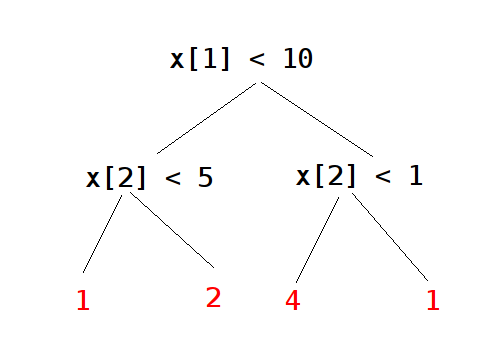
\includegraphics[width=10cm]{img/d_tree}
\end{center}
\caption{Решающее дерево: в узлах предикаты, в листьях значения целевой функции}
\label{d_tree}
\end{figure}

\subsubsection{Метод опорных векторов}
Метод опорных векторов основан на \textbf{принципе максимизации зазора}. Пусть стоит задача классификации с двумя классами. В пространстве признаков классифицируемых объектов проводится гиперплоскость таким образом, чтобы объекы обучающей выборки принадлежащие одному классу лежали по одну сторону от этой гиперплоскости, а объекты принадлежащие второму классу по другую.

Понятно, что если гиперплоскость существует, то она не единственна. Среди всех таких гиперплоскостей выбирается такая, которая максимизирует \textbf{зазор} -- минимальное расстояние от гиперплоскости до ближайшей точки обучающей выборки. Таким образом расстояние от гиперплоскости до ближайшего объекта каждого из классов будет одинаково.

\begin{figure}[h]
\begin{center}
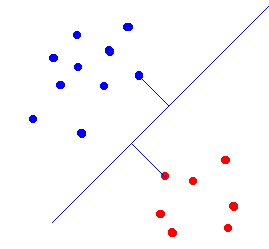
\includegraphics[width=5cm]{img/svm}
\end{center}
\caption{Наилучшая разделяющая прямая в двухмерном пространстве}
\label{svm}
\end{figure}

Если разделяющая гиперплоскость существует выборка называется \textbf{линейно разделимой}.

Для обобщения на случай линейно неразделимой выборки используется следующая идея: выборку можно сделать линейно разделимой, если увеличить размерность пространства. Для этого используется так называемая \textbf{ядерная функция}

\begin{figure}[h]
\begin{center}
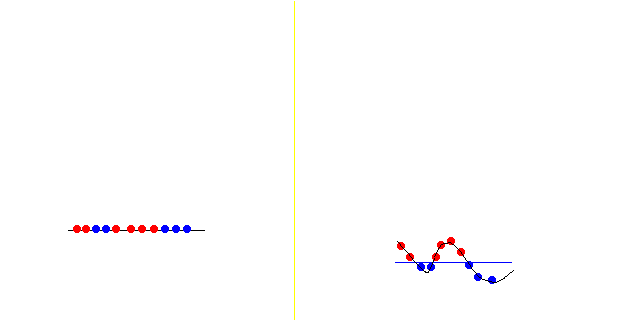
\includegraphics[width=15cm]{img/svm2}
\end{center}
\caption{Неразделимая в одномерном пространстве выборка стала разделимой после перевода в двумерное пространство}
\label{svm-kernel}
\end{figure}

Метод опорных векторов в настоящее время рассматривается как наиболее универсальный и хорошо работающий на большом количестве задач. Кроме того в работе А. Розинкина было показано что этот метод показывает хорошие результаты при применении его к задаче фильтрации спама. Для решения поставленной задачи мы также воспользуемся этим методом.

\subsection{Обзор существующих открытых систем фильтрации спама}
По требованию постановки задачи реализация должна быть выполнена в виде модификации одной из существующих систем фильтрации спама. В данном разделе будут приведены описания некоторых систем фильтрации спама и выбрано одно из них для дальнейшей модификации. 

\textbf{spamassassin}

SpamAssassin - одно из наиболее известных открытых средств фильтрации спама. Этот проект динамично развивается и показывает хорошие результаты производительности и качества фильтрации. SpamAssassin использует в своей работе большое количество методик обнаружения спама.

\textbf{spamprobe}

Система Spamprobe написана на языке C++ и использует байесовский подход к фильтрации спама. В настоящее время практически не поддерживается, последняя версия была выпущена в 2007 году.

\textbf{bogofilter}

Система работает на стороне клиента, может интегрироваться в различные почтовые клиенты(такие как kmail и evolution). Использует в своей работе байсовские методы.

\textbf{bmf}

Очень маленький по размеру (около 4000 строк кода) спам-фильтр. Использует байесовский подход к фильтрации спама. в настоящее время не поддерживается.

\textbf{Quick Spam Filter}

Использует байесовский подход к фильтрации спама. Написан на языке C, в связи с чем работает достаточно быстро. В настоещее время не поддерживается.

\textbf{scmail}

Написан на языке scheme. Для фильтрации использует различные эвристическии подходы. В настоящее время не поддерживается.

\textbf{Spambayes}

Написан на языке python, поэтому достаточно прост в модификации. Работает на стороне почтового клиента.

\textbf{dspam} - открытая система фильтрации спама. Dspam изначально проектриовался для работы в многопользовательском режиме.
Для фильтрации спама dspam может использовать одну из нескольких разновидностей байесового классификатора.
Dspam написан на языке С и работает достаточно эффективно. Dspam имеет большое сообщество разработчиков и активно развивается в настоящий момент.
Из недостатков системы dspam можно отметить использование устаревшей системы сборки (autools) и использование низкоуровневой разработки, что усложняет понимание и модификацию его исходного кода.
\begin{figure}[h]
\begin{center}
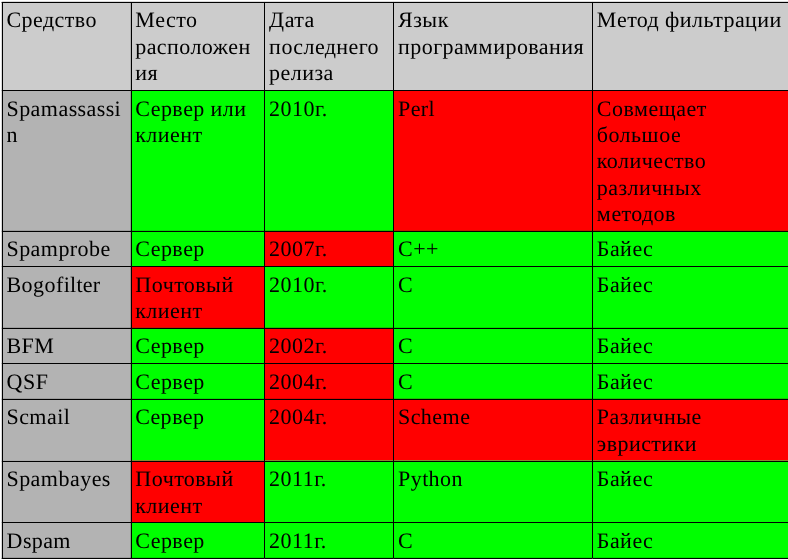
\includegraphics[width=13cm]{img/compare}
\end{center}
\caption{Сравнение систем фильтрации спама}
\label{spam_systems}
\end{figure}


Для доработки был выбран именно dspam, так как он удовлетворяет нашим требованиям, а именно:
\begin{itemize}
\item Ориентирован на работе на стороне сервера
\item Распространяется под свободной лицензией
\item Ориентирован на многопользовательский режим
\item Фильтрация спама осуществляется  всего одним алгоритмом, что упрощает тестирование разработанного метода
\end{itemize}


\newpage
\section{Исследование и построение решения задачи}
\label{research}
% В разделе «Исследование и построение решения задачи» должна быть проведена 
% декомпозиция исходной задачи на последовательность подзадач, которые нужно 
% решить для получения решения исходной задачи, приведены обосновании всех 
% принимаемых решений. Например, если принимается решение о создании некоторого 
% программного средства, то необходимо показать, что не существует средства, 
% обладающего нужными характеристиками. Исключение составляет случай, когда 
% такое средство создается в учебных целях. Обоснование может быть дано одним 
% из следующих способов:
% 1.Экспертный: приводятся высказывания, мнения авторитетных специалистов, с 
% указанием ссылок на источники, где оно сформулировано;
% 2.Дедуктивный: яркий пример математика - есть система аксиом и правил вывода. 
% Если ты сумел показать, как вывести свое утверждение из аксиом с помощью 
% правил вывода, то все обосновано.
% 3.Естественнонаучный: выдвигается 
% гипотеза (то, что обосновываем) и проводится серия экспериментов, на основании 
% обработки результатов этих экспериментов гипотеза либо подтверждается, либо нет
% 4. Инженерно-практический:  хорош когда в качестве утверждения выступает некий 
% принцип или система, работоспособность которого мы хотим обосновать, тогда 
% экспериментальная реализация может выступать в качестве обоснования.. 

Задача классификации данных лазерной локации сводится к задаче классификации прецедентов, образующих связные множества, путем выполнения подготовительных этапов: загрузки данных, обеспечения быстрого доступа к ним, определения используемых признаков и их вычисления. Эти подготовительные этапы являются специфичными для задачи. В отличии от них, этапы классификации и выделения объектов универсальны, поэтому сформулированы в терминах прецедентов и связных областей.

\subsection{Загрузка данных}

На сегодняшний день существует два распространенных формата хранения данных лазерной локации: LAS и текстовый. Чаще всего используется текстовый формат, представляющий из себя CSV\footnote{Значения перечислены через точку с запятой, записи разделены переносами строк} в котором заданы координаты и яркости точек\footnote{Точное число полей и их содержание зависит от модели и производителя оборудования}. Главными недостатками этого формата являются крайне неэффективное хранение данных и непостоянная длинна записи, что исключает возможность чтения файла с произвольного места. Альтернативой является стандарт LAS, хранящий данные в бинарном виде и имеющий фиксированную длину записи. Кроме того стандарт LAS определяет набор классов, к которым может принадлежать точка, впрочем предусмотрена возможность использования собственного набора классов. В виду простоты конвертации текстовых данных в LAS и наличия библиотеки для работы с ним именно этот формат был выбран в качестве входного.

Данные лазерной локации могут содержать миллионы точек, а для вычисления коллективных признаков необходимо быстро находить все точки, расположенные в некотором ограничивающем объеме. В литературе предлагается два решения: регуляризация данных и KD-деревья. Регуляризация заключается в рассмотрении данных как псевдотрехмерных, после чего точки выравниваются по равномерной двумерной сетке\cite{Amin}. Недостающие значения интерполируются и данные заносятся в двумерный массив. Таким образом обеспечивается обращение по координатам и поиск соседей за константное время. Однако этот метод не применим для трехмерных данных, и приводит к большим накладным расходам или неточностям в случае неравномерности распределения точек. К сожалению даже данные авиационной лазерной локации не всегда удовлетворяют этим условиям. KD-деревья более универсальны и могут быть использованы для любых данных. В итоге было выбрано комбинированное решение: данные делятся на блоки, хранящиеся в многомерном массиве, а внутри блока точки хранятся в KD-дереве. Это позволяет снизить высоту деревьев на несколько уровней, но главное преимущество такого решения заключается в возможности использования блоков для поточной классификации.

Для каждого блока определяется, какие соседние блоки необходимы для вычисления коллективных признаков точек блока. Когда поступают все необходимые соседние блоки, блок ставится в очередь на классификацию. Также возможна повторная классификация блока, если поступила дополнительная информация для него или его соседей. Кроме того, добавление нового блока не приводит к балансировке деревьев в других блоках, такая локальность изменений позволяет параллельно получать и обрабатывать данные.

\subsection{Выделение объектов}

Как было сказано в обзоре, в настоящий момент объекты, как правило, выделяют исходя из геометрических соображений.
Предлагается вместо специализированной процедуры выделения объектов использовать методы классификации с последующим выделением связных областей, имеющих один и тот же класс. Такой подход позволяет выделять соприкасающиеся объекты разных классов и объекты, не выделяющиеся своей формой, более того, он может применяться и в случае, если не определено расстояние между прецедентами или это расстояние не является мерой. Также возможно представление объектов как нечетких множеств прецедентов. Единственным условием применимости данного подхода является наличие алгоритмов классификации прецедентов.

После выделения объектов становится возможно введение дополнительных признаков, явное использование объектов в алгоритмах классификации и уточнение областей, по которым вычисляются коллективные признаки. Если коллективный признак обладает свойством аддитивности, то он может вычисляться по формуле
$$
F_c=\sum_{p \in N}\sum_{i \in C}\sum_{j \in C}(F^p \cdot p_i \cdot p_j^p)
$$
\begin{ESKDexplanation}
\item[где ] $F_c$ "--- скорректированное значение признака;
\item $N$ "--- множество прецедентов, принадлежащих окрестности прецедента, для которого вычисляется признак;
\item $C$ "--- множество допустимых классов;
\item $F^p$ "--- вклад в признак прецедента $p$;
\item $p_i$ "--- вероятность того, что прецедент, для которого вычисляется признак, имеет класс $i$;
\item $p_j^p$ "--- вероятность того, что прецедент $p$ имеет класс $j$.
\end{ESKDexplanation}

\subsection{Классификация}

Для реализации вышеописанного алгоритма требуется проведение как минимум двух этапов классификации. Но для повышения точности количество этапов может быть увеличено: на различных этапах могут применяться разные наборы классов, производиться отсев заведомо ошибочных объектов, вычисление и уточнение значений коллективных признаков. Поэтому вместо применения фиксированной последовательности алгоритмов предлагается ввести понятие \textbf{многоэтапной классификации}. 

Из операций классификации, оценки зависимостей и иных действий над данными строится ациклический ориентированный граф. Этапом называется выполнение одного из действий, результатом которого является вычисление новых свойств прецедентов, уточнение уже имеющихся свойств или добавление/удаление прецедентов. На каждом этапе доступны все данные, полученные на предыдущем этапе, что позволяет вычислять и использовать взаимосвязи между прецедентами. Состав классов и тип прецедентов может меняться по ходу вычисления.
%TODO вставить картинку с этапами

Соответственно возникает потребность в создании создание программного средства, обеспечивающего такой процесс классификации. Оно должно обеспечивать построение графа классификации пользователем, хранение промежуточных данных (прецедентов) в предметно-независимом виде, передачу данных для обработки алгоритмам, обеспечивающим выполнение этапов, и обучение алгоритмов классификации, реализующих отдельные этапы.

\subsubsection{Обучение многоэтапного классификатора}

Благодаря отсутствию циклов в графе классификации, в случае использования жадной стратегии\footnote{То есть на каждом этапе алгоритмы классификации обучаются на получение наилучшей точности на своем этапе.}, он может быть обучен за один проход сверху-вниз. Для обучения необходимо иметь обучающую выборку, состоящую из прецедентов и назначенных им классов, для каждого их этапов. Обучающая выборка состоит из двух компонент: набора прецедентов и назначенных им классов. В данном случае эти компоненты разделяются: назначенные классы пользователь должен задать для каждого этапа отдельно\footnote{Для всех этапов, на которых список допустимых классов и тип прецедентов совпадают, назначенные классы могут быть заданы одинаковыми.}, а набор прецедентов задается только для первого этапа. Этих данных достаточно для обучения первого этапа. После обучения каждого очередного этапа производится классификация прецедентов обучающей выборки и полученные данные используются для обучения следующего этапа.

\subsubsection{Классификация данных лазерной локации}

Для проведения многоэтапной классификации данных лазерной локации предлагается ввести операции, перечисленные на рисунке \ref{stages}. Специфичными для данной задачи являются модули генерации признаков и специализированные алгоритмы фильтрации, удаляющие одиночные ошибки. Модули генерации признаков можно разделить на две категории: модули для выделения коллективных признаков из множеств прецедентов (список признаков такого типа приведен в приложении \ref
{local properties}) и модули генерации признаков, обеспечивающих передачу информации между этапами.

Использование признаков, описывающих классы близлежащих прецедентов, позволяет учитывать зависимости между ними в методах классификации независимых прецедентов, скорость которых выше скорости работы алгоритмов, учитывающих зависимости в явном виде.

\begin{figure}[t]
\begin{center}
\includegraphics{img/stages}
\end{center}
\caption{Типы операций, используемые при многоэтапной классификации данных лазерной локации}
\label{stages}
\end{figure}

%Декомпозиция задачи. Входные данные - LAS + конвертеры, обосновать почему LAS. Вычисление первичных признаков, определение и вычисление сводных признаков. Классификация. Возможность классификации потока информации. Идея многоэтапной классификации.

%TODO создание обучающих наборов, если будет не хватать объема
\newpage
\section{Реализация}

% Если в рамках работы проводится реализация некоторого программного средства,
% то в разделе «Описание практической части» обязательно должна быть описана
% его программная реализация, в частности:
% приведены обоснования выбранного инструментария;
% приведена с иллюстрацией общая архитектура разработанного средства;
% приведена с иллюстрацией схема работы средства;
% если осуществляется доработка существующего средства, то должны быть описаны
% новые возможности/улучшения, реализованные в данной работе.
% обязательно должны быть приведены характеристики функционирования (например,
% сложность, производительность, время реакции и т.д.)
\subsection{Библиотека libsvm}
Библиотека libsvm содержит реализацию метода опорных векторов. Она содержит интерфейсы для построения моделей по обучающей выборки и предсказания значения целевой функции по  существующей модели. Дополнительно эта библиотека содержит интерфейсы для сохранения модели в файл и загрузки ее из файла.

Для создания модели можно пользоваться несколькими ядровыми функциями(линейная, полиномиальная, сигмоид и другие), а также задавать все необходимые для работы метода параметры.

Кроме того можно указывать тип решаемой задачи: классификация, классификация с двумя классами, регрессия и др.

Существует версия библиотеки libsvm использующая современные графические процессоры, логика работы в которой написана на CUDA. Использование графических процессоров позволяет существенно уменьшить время построения модели и время предсказания(смотри график).

Вместе с библиотекой поставляются некоторое количество исполняемых файлов, которые позволяют строить модель по данным из файла в определенном формате, а также осущесвлять предсказание для даннах записанных в файле по построенноей модели. Также поставляется некоторое количество тестовых данных.

\subsection{Архитектура dspam}
В основе dspam лежит библиотека libdspam, которая реализует логику фильтрации.
Эта библиотека содержит код нескольких алгоритмов фильтрации (одновременно использоваться может только один из них)
Кроме того библиотека содержит несколько вспомогательных классов реализующих некоторые структуры данных(списки, деревеья и т. п), а также драйвер хранилища данных.

Данные могут храниться либо в одной из поддерживаемых СУБД(это MySQL, Posgres и SQLite), а также непосредтсвенно в файловой системе(используется собственная методика хранения пар ключ-значение).

\begin{figure}[h]
\begin{center}
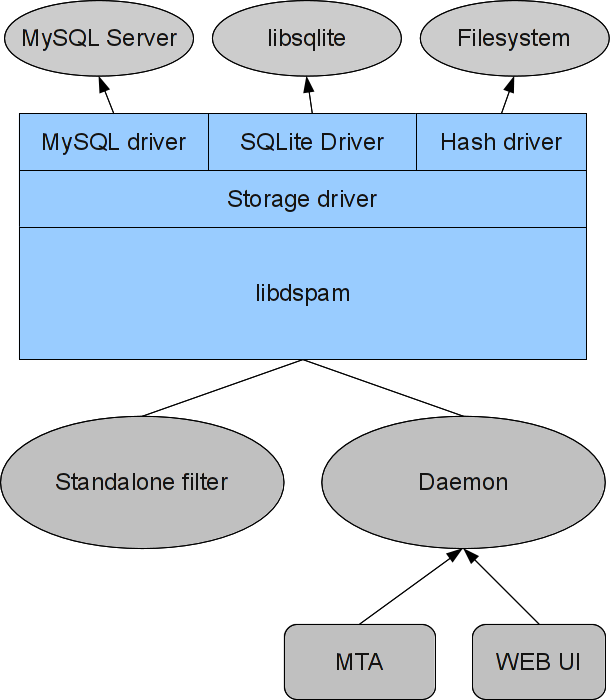
\includegraphics[width=10cm]{img/dspamarch}
\end{center}
\caption{Архитектура dspam}
\label{dspamarch}
\end{figure}

Dspam может работать либо в режиме standalone-фильтра, либо демона. В обоих случаях
исполняемый модуль линкуется с библиотекой libdspam.

Работа в standalone режиме подразумевает что бинарный файл запускается по требованию. Тестируемое письмо в этом случае подается исполняемому модулю на стандартный вход, а информацию о произведенном тестировании можно
получить со стандартного вывода. Эта информации может быть представлена в виде короткой строчки в которой содержится класс, к которому отнес классификатор письмо и вероятностью или в виде самого письма с установленными заголовками. Этот режим удобно использовать для тестирования системы, а так же в случае кода количество писем достаточно мало и требование к производительности невелики.

Работа в режиме демона подразумевает что исполняемый код постоянно находится в оперативной памяти. Общение с клиентом в этом случае происходит либо через сеть (используется tcp-сокет), либо через UNIX-сокет. Таким образом dspam в этом случае является полноценным серверным приложением. Сервер по запросу от клиента принимает письмо, классифицирует, проставляет необходимые заголовки и возвращает клиенту. Клиентом в таком случае выступает система доставки почты(MTA).

Кроме того сервер может выполнять некоторые сервисные команды: просмотр статистики, очистка хранилища данных и т. п. В этом случае клиентом может быть например web-интерфейс администратора.


\subsection{Модификация dspam}
Для обеспечения работы описанного в разделе \ref{research} метода была произведена модификация библиотеки libdspam: в функцию обработки письма был добавлен код, который при определенных настройках вызывает функцию обработки письма нашим методом.

Функция обработки обрабатывает уже разбитое на токены письмо. Для разбития письма на токены используется встроенная в dspam функциональность. В зависимости от режима работы(обучение или классификация) вызывается одна из двух функций.

Функция обучения записывает в файл информацию об адресате письма и частотах токенов. По этому файлу в последствии строится модель для метода опорных векторов

Функция классификации загружает из файла уже построенную модель, строит вектор с частотами и вычисляет вероятности.

\subsection{Схема работы}
Опишем схему работы разработанного средства в различных случаях.
\begin{figure}[h]
\begin{center}
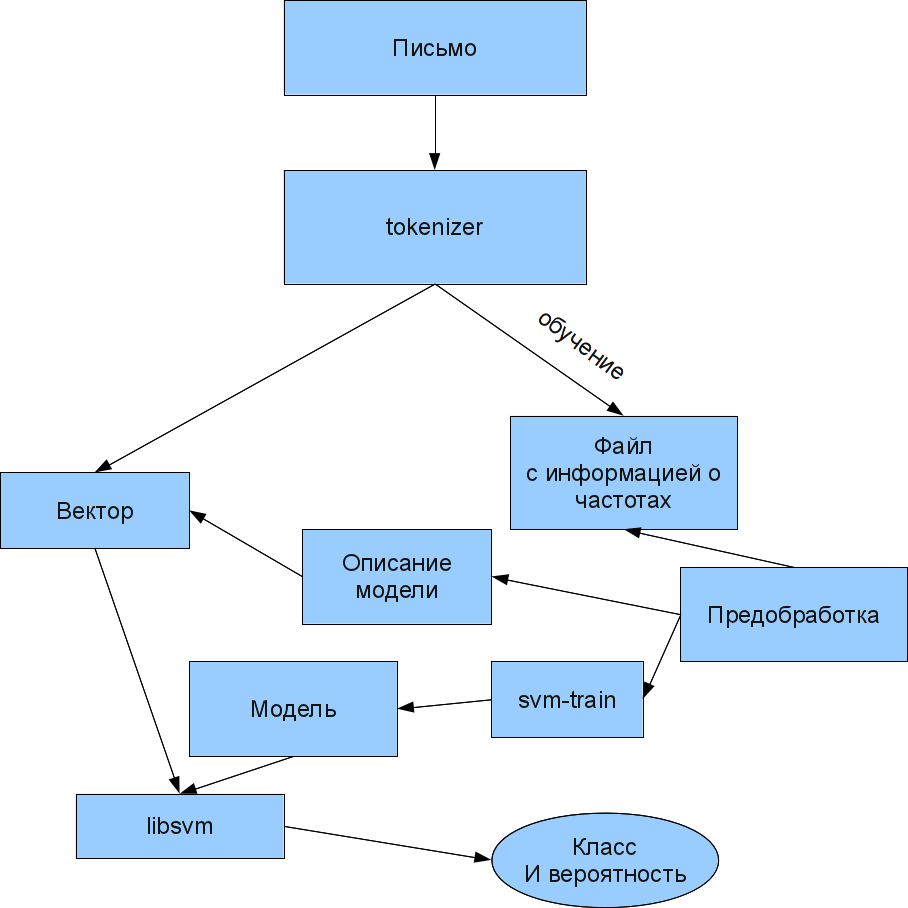
\includegraphics[width=12cm]{img/working_scheme}
\end{center}
\caption{схема работы классификатора}
\label{dspamarch}
\end{figure}

\subsubsection{Добавление письма в обучающую выборку}

\begin{enumerate}
    \item Письмо попадает в систему.
    \item Выясняется адресат письма.
    \item Письмо разбивается на токены.
    \item Вычисляются частоты токенов.
    \item Информация о классе письма, адресате и частотах токенов записывается в файл частот.
\end{enumerate}

\subsubsection{Построение модели}
\begin{enumerate}
    \item Вызывается скрипт построения модели (вызов происходит раз в день при помощи стандартной службы CRON).
    \item Вычисляются общие частоты токенов для каждого токена из файла частот.
    \item Выбираются наиболее употребимые токены (токены с наибольшей частотой).
    \item Для каждого из писем строится вектор, содержащий частоты наиболее употребимых токенов, а также индикаторы принадлежности письма пользователю (все кроме одного индикаторы равны нолю).
    \item Построенное множество векторов записывается во временный файл вместе с информацией о классах писем,  соответсвующих векторам.
    \item По построенному временному файлу генерируется модель при помощи инструмента svm-train.
    \item Информация о токенах используемых для построения модели сохраняется во временный файл описания модели.
\end{enumerate}

\subsection{Классификация}
\begin{enumerate}
    \item Письмо попадает в систему.
    \item Выясняется адресат письма.
    \item Письмо разбивается на токены.
    \item Вычисляются частоты токенов.
    \item Загружается описание модели
    \item По описанию модели, адресату и частотах токенов строится вектор
    \item Загружается модель
    \item По модели и вектору вычисляется вероятность принадлежности письма спаму
    \item По пороговому правилу выставляется оценка спам/не спам
\end{enumerate}

\subsection{Описание проведенных экспериментов}

\section{Экспериментальное исследование}

Для экспериментальной проверки разработанного программного средства были проведены две серии экспериментов. Первая серия проведена для сравнения разработанного программного средства с наивным байесовским классификатором, используемым во многоих открытых системах фильтрации спама.

Вторая серия экспериментов проведена для проверки работы системы в многопрофильном режиме.

\subsection{Сравнение с наивным байесовским классификатором}

\subsubsection {Набор данных}

Тестирование производилось на двух публичных наборах email-сообщений.

\begin{enumerate}
	\item SpamAssassin public corpus \cite{SAPC}
	\item CEAS 2008 Live Spam Challenge Laboratory Corpus \cite{CEAS}
\end{enumerate}

\subsubsection{Методика тестирования}

Тестирование производилось с использованием метода скользящего контроля: выборка разбивалась на пять частей, на четырех из которых проводилось обучение, а на пятой - контроль. Выборка \cite{CEAS} ввиду своей большой величины была разделена на несколько частей, на каждой из которых тестирование было произведено отдельно. 

Результат тестирования представлен в виде графика соответствия величин вероятности ложно-положительного срабатывания и вероятности верного обнаружения спама. Точка на графике обозначает что при определенной границе решающего правила система будет работать именно в таком режиме: фильтровать спам с вероятностью показанной на оси ординат и классифицировать легитимные письма как спам с вероятностью показанной на оси абцисс. Чем выше проходит график, тем более качественно работает система фильтрации.

\subsubsection{Результаты тестирования}
На графиках \ref{SAPCBAYESSVM} и \ref{CEASBAYESSVM} представлены результаты тестирования на наборах \cite{SAPC} и \cite{CEAS}. Видно, что разработанное средство всегда работает лучше чем наивный байесовский классфикатор.

\begin{figure}[h]
\begin{center}
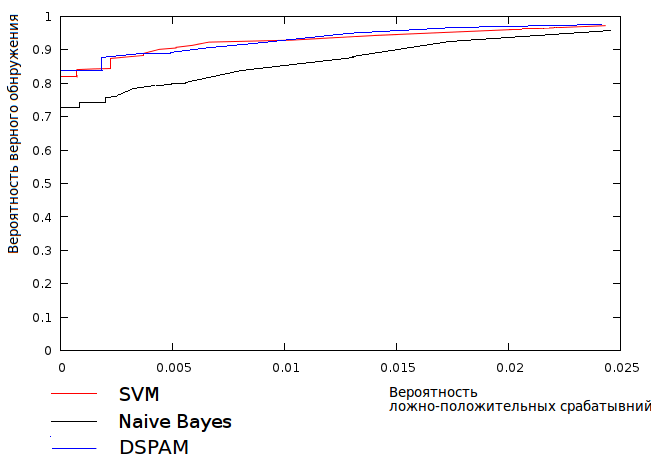
\includegraphics[width=15cm]{img/graphic}
\end{center}
\caption{Сравнение качества тестирования реализованного алгоритма и наивного байесовского классификатора на наборе \cite{SAPC}}
\label{SAPCBAYESSVM}
\end{figure}

\begin{figure}[h]
\begin{center}
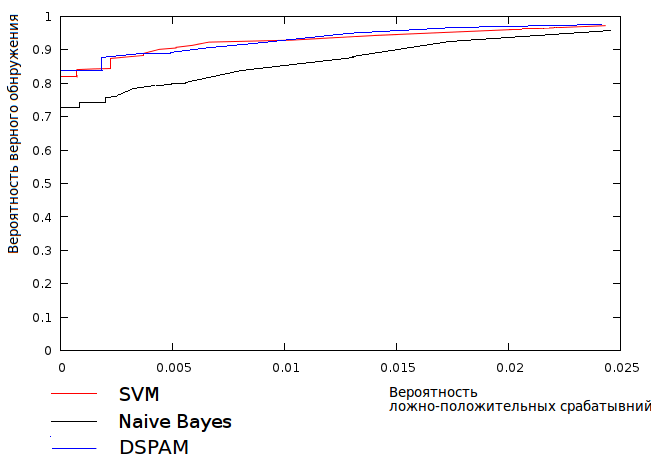
\includegraphics[width=15cm]{img/graphic}
\end{center}
\caption{Сравнение качества тестирования реализованного алгоритма и наивного байесовского классификатора на наборе \cite{SAPC}}
\label{CEASBAYESSVM}
\end{figure}

\subsection{Тестирование работы в многопрофильном режиме}

\subsubsection{Набор данных}
Тестирование производилось на наборе данных SpamAssassin Public Corpus \cite{SAPC}.
Для проведения эксперимента сообщения, представленные в выборке были разделены на 3 класса:
\begin{enumerate}
\item Класс, сообщения из которого все письма считаются легитимной почтой.
\item Класс, сообщения из которого все пользователи считают спамом
\item Класс, сообщения из которого считают спамом некоторые из пользователей
\end{enumerate}

В класс 1 были включены все сообщения, отмеченные в наборе \cite{SAPC} как спам. Классы 2 и 3 были получены из писем, отмеченных в наборе \cite{SAPC} как легитимная почта.
\begin{enumerate}
	\item Эксперимент показывающий, что новые добавление пользователей не ухудшает качество фильтрации.

	Для проведения эксперимента использовались классы писем 1 и 2. Каждый из классов был поделен случайным образом на две части. Эти части считались обучающими выборками для двух разных пользователей. Далее было произведена проверка метода при помощи скользящего контроля, с учетом того, что в системе теперь не один а два пользователя.

	\item Эксперимент показывающий что многопрофильность работает, и обучение на данных одного пользователя распространяется на другого. Сообщения из всех трех классов были разделены на две части(для первого и второго пользователей). Обучение производилось на всех трех наборах для первого пользователя и на первых двух для второго. Далее было произведено тестирование второго пользователя на сообщениях из третьей группы и посчитаны оценкивероятности принадлежности к спаму для писем. На результируещем графике показаны диапазоны вероятности и количество писем попавших в этот диапазон.

	\item Эксперимент показывающий что разное мнение пользователей о группе писем не приводит к проблемам. Эксперимент аналогичен предыдущему, за исключением того, что второй пользователь также обучался на письмах из третьей группы. На результирующем графике представлены диапазоны вероятности и количество писем попавших в этот диапазон для первого и второго пользователей. 
	
\end{enumerate}
\subsubsection{Результаты}


\newpage
\section{Заключение и результаты}

% Заключение (не более чем на 1 страницу) должно содержать краткую формулировку 
% результатов работы, выносимых на защиту и согласованных с целью работы. 

\begin{itemize}
  \item Проведено исследование особенностей применения методов машинного обучения к задаче классификации прецедентов, образующих связные множества
  \itemПредложен способ улучшения качества классификации путем  комбинирования методов классификации и более точного учета зависимостей классов связных прецедентов
  \itemРеализована система многоэтапной классификации. Тестирование на данных лазерной локации показало повышение качества классификации по сравнению с классическими алгоритмами
\end{itemize}

На основании проведенных тестов можно утверждать, что предложенный способ позволяет увеличить точность и уменьшить количество одиночных ошибок, что облегчает дальнейшую обработку результатов классификации.
\section{Приложение}
\begin{longtable}{|l|l|l|}
\caption[Апробация на реальных данных]{Апробация на реальных данных}  \label{REALDATATABLE} \\
День & Верные срабатывания & ложно-положительные срабатывания  \\  
2 & 0.997175141243 & 0.0 \\
3 & 0.991176470588 & 0.00833333333333 \\
4 & 0.988023952096 & 0.00724637681159 \\
5 & 0.988826815642 & 0.0 \\
6 & 0.993846153846 & 0.0382165605096 \\
7 & 0.968208092486 & 0.0 \\
8 & 0.990909090909 & 0.0 \\
9 & 0.984802431611 & 0.0 \\
10 & 1.0 & 0.00787401574803 \\
11 & 0.994505494505 & 0.0298507462687 \\
12 & 0.994750656168 & 0.0 \\
13 & 0.98275862069 & 0.0 \\
14 & 0.997084548105 & 0.0220588235294 \\
15 & 0.990963855422 & 0.00662251655629 \\
16 & 0.992518703242 & 0.0 \\
17 & 0.997229916898 & 0.00704225352113 \\
18 & 0.997159090909 & 0.0 \\
19 & 0.994350282486 & 0.00757575757576 \\
20 & 0.997326203209 & 0.0 \\
21 & 0.994047619048 & 0.0 \\
22 & 0.997142857143 & 0.00854700854701 \\
23 & 1.0 & 0.0 \\
24 & 0.997191011236 & 0.00724637681159 \\
25 & 0.994202898551 & 0.00826446280992 \\
26 & 0.994011976048 & 0.008 \\
27 & 0.997395833333 & 0.0 \\
28 & 1.0 & 0.0 \\
29 & 0.997126436782 & 0.0149253731343 \\
30 & 0.997014925373 & 0.0 \\
\end{longtable}
 

\newpage
\begin{thebibliography}{99}
%\bibitem{Amin}Amin P. Charaniya, Roberto Manduchi, Suresh K. Lodha Supervized Parametric Classification of Aerial
%\bibitem{Markov random fields}Dragomir Anguelov, Ben Taskar, Vassil Chatalbashev, Daphne Koller, Dinkar Gupta, Geremy Heitz, Andrew Ng LiDAR Data Discriminative Learning of Markov Random Fields for Segmentation of 3D Scan Data 2005
%\bibitem{MMM}Anuraag Agrawal, Atsushi Nakazawa, Haruo Takemura MMM-classification of 3D Range Data 2009
%\bibitem{full waveform}Clement Mallet, Uwe Soergel, Frederic Bretar ANALYSIS OF FULL-WAVEFORM LIDAR DATA FOR CLASSIFICATION OF URBAN AREAS 2006
%\bibitem{filer comparison}George Sithole, George Vosselman Report: ISPRS Comparison of Filters 2003
%\bibitem{whole objects}D. Tóvári, T. Vögtle CLASSIFICATION METHODS FOR 3D OBJECTS IN LASERSCANNING DATA
%\bibitem{Brenner}Claus Brenner Aerial Laser Scanning 2006
%\bibitem{growing}Gianfranco Forlani, Carla Nardinocchi ADAPTIVE FILTERING OF AERIAL LASER SCANNING DATA 2007
%\bibitem{national dataset}Developments of National Lidar Dataset, ASPRS 2009 Annual Meeting, Baltimore, Maryland
%\bibitem{RDN} Jennifer Neville, David Jensen Relational Dependency Networks 2007
%\bibitem{flood} USGS - Flood Mapping Research [HTML] http://wa.water.usgs.gov/projects/pugethazards/urbanhaz/MappingNWS.htm

%\bibitem{full waveform rus}Andreas Ulrich, Nikolaus Studnicka, Markus Hollaus, Cristian Briese, Wolfgang Wagner, Michael Doneus и Werner Mucke Улучшение цифровой модели рельефа за счет полной волновой картины, полученной при лазерном сканировании 2007г.
%\bibitem{vegetation mapping}Vesna Ducic, Markus Hollaus, Andreas Ullrich, Wolfgang Wagner и Thomas Melzer 3D VEGETATION MAPPING AND CLASSIFICATION USING FULL-WAVEFORM LASER SCANNING 2006
%\bibitem{weka}Домашняя страница проекта WEKA [HTML] http://www.cs.waikato.ac.nz/~ml/

%\bibitem{SMAP}Документация по классификации пакета GRASS [HTML] http://grass.osgeo.org/grass64/manuals/html64\_user/i.smap.html
\end{thebibliography}


\end{document}
% vim:tw=70
